%===============================================================================
%===============================================================================
%
\clearpage
%
\subsection{Example-0111 \texttt{[CONVERGES]}}
%
%===============================================================================
%
\subsubsection{Mathematical model}
%
We solve the following equation,
%
\begin{align}
    \nabla \cdot \boldsymbol{\sigma} (\boldsymbol{u}, t) = \boldsymbol{0} & &&\Omega = [0, 160] \times [0, 120], t \in [0, 5],
\end{align}
%
with time step size $\Delta_t = 1$ and boundary conditions
%
\begin{align}
    \ldots & && \ldots, \\
    \ldots & && \ldots.
\end{align}
%
2D: specify thickness, Young's modulus and Poisson's ratio.
%
%===============================================================================
%
\subsubsection{Computational model}
%
\begin{itemize}
    \item{Length, width, height}
    \item{Direct/iterative solver}
    \item{Generated/user mesh}
    \item{Number of elements}
    \item{Interpolation order}
    \item{Number of solver steps (time steps, load steps)}
\end{itemize}
%
%===============================================================================
%
\subsubsection{Results}
%
\begin{figure}[h!]
    \centering 
    \includegraphics[width=\columnwidth]{examples/example-0101/doc/figures/analytical_solution.eps} 
    \caption{Results, analytical solution.}
    \label{example-0101-analytical-solution-fig}
\end{figure}
%
\begin{figure}[h!]
    \centering 
    \includegraphics[width=\columnwidth]{examples/example-0101/doc/figures/abaqus_reference.eps} 
    \caption{Results, Abaqus reference.}
    \label{example-0101-abaqus-reference-fig}
\end{figure}
%
\begin{figure}[h!]
    \centering 
    \includegraphics[width=\columnwidth]{examples/example-0101/doc/figures/iron_reference.eps} 
    \caption{Results, iron reference.}
    \label{example-0101-iron-reference-fig}
\end{figure}
%
\begin{figure}[h!]
    \centering 
    \includegraphics[width=\columnwidth]{examples/example-0101/doc/figures/current_run.eps} 
    \caption{Results, current run.}
    \label{example-0101-current-run-fig}
\end{figure}
%
%===============================================================================
%
\subsubsection{Validation}
%
CHeart rev.\ 6328, Abaqus 2017, analytical reference solution, whatever...
%
%===============================================================================
%===============================================================================
